% 注释要用%开头,只提供整行注释

\documentclass[UTF8]{article} % 这句限制了整个文档的类型
% 类型就是包括标题啊章节啊等等在内的一套设定
% 比如你想写一个类似论文的东西,就用article就好了
% 前面的UTF8是编码方式
% 注意 反斜杠\后面的是函数,函数值中暂时可以认为调整参数写在[中括号里],内容在{大括号里}

\usepackage[zihao=-4]{ctex} % ctex可以写中文,中括号里那句的意思是正文小四号
\usepackage[a4paper]{geometry} % 调整纸张大小和页边距的包,这里中括号中规定了纸张大小
\usepackage{graphicx} % 用它在报告里加图
\usepackage{float}
\usepackage{indentfirst} % 用于首行缩进
\usepackage{listings}	% 代码插入
\usepackage{matlab-prettifier} % matlab 代码插入美化
\usepackage{url}

\geometry{left=2.0cm,right=2.0cm,top=2.0cm,bottom=2.0cm} % 页边距设置
\setlength{\parindent}{2em} 	% 首行缩进2个中文字符

% 设置中英文摘要
%\newcommand{\enabstractname}{Abstract}
%\newcommand{\cnabstractname}{摘要}
%\newenvironment{enabstract}{%
%	\par\small
%	\noindent\mbox{}\hfill{\bfseries \enabstractname}\hfill\mbox{}\par
%	\vskip 2.5ex}{\par\vskip 2.5ex}
%\newenvironment{cnabstract}{%
%	\par\small
%	\noindent\mbox{}\hfill{\bfseries \cnabstractname}\hfill\mbox{}\par
%	\vskip 2.5ex}{\par\vskip 2.5ex}


% tile author date
%\title{电动汽车BMS设计与数字孪生的研究}
%\author{周密}
%\date{\today}

\begin{document}
	%% 封面设计
	% logo 中南大学
	\vspace*{1cm}
	\begin{figure}[htbp]
		\centering
		\graphicspath{{./images/}}
		
\includegraphics[width=0.7\linewidth]{logo}
	\end{figure}
	\vspace*{0.5cm}
	
	% 标题居中显示
	\begin{center}
		\Huge{\textbf{数字图像处理课程实验报告}}
	\end{center}
	
	\vspace*{3.5cm}
	% 信息表格
	\begin{table}[h]
		\centering
		\begin{Large}
			\begin{tabular}{p{3cm} p{6cm}}
				姓\qquad 名:&  周密 \\
				\hline
				学\qquad 院:&  计算机学院\\
				\hline
				学\qquad 号:&  8210182308 \\
				\hline
				邮\qquad 箱: & zhoumicsu@csu.edu.cn\\
				\hline
				指导老师:&  唐艳\\
				\hline
				日\qquad 期:&  2021年11月27日晚 \\
				\hline
			\end{tabular}
		\end{Large}
	\end{table}
	\thispagestyle{empty}       %本页不显示页码
	
	\clearpage
	%% title
	%\maketitle
	
	%% 摘要
	%	\begin{cnabstract}
	
	%		\par\textbf{关键词: } 锂离子电池; 电动汽车; 电池管理系统; BMS; 电池数据分析; MATLAB APP Designer%“\par在段首,表示另起一行,“\textbf{}”,花括号内的内容加粗显示
	%	\end{cnabstract}
	%	\begin{enabstract}	
	%		\par\textbf{Keywords:} Lithium-ion battery; Electric vehicle; Battery management system; Battery data analysis; MATLAB APP Designer
	%	\end{enabstract}
	%	\thispagestyle{empty}       %本页不显示页码
	%	\clearpage
	
	%% 目录
	\tableofcontents
	\thispagestyle{empty}       %本页不显示页码
	\clearpage
	
	\setcounter{page}{1}        %从下面开始编页,页脚格式为导言部分设置的格式
	%% 正文内容
	
	\section{实验一:数字图像的基本操作和灰度变换}
	\subsection{实验目的}
	1. 了解数字图像的基本数据结构
	
	2. 熟悉Matlab中数字图像处理的基本函数和基本使用方法
	
	3. 掌握图像灰度变换的基本理论和实现方法
	
	4. 掌握直方图均衡化增强的基本理论和实现方法
	
	\subsection{实验原理}
	1. 图像灰度的线性变换
	
	灰度的线性变换可以突出图像中的重要信息。通常情况下,处理前后的图像灰度级是相同的,即处理前后的图像灰度级都为$[0,255]$。那么,从原理上讲,我们就只能通过抑制非重要信息的对比度来腾出空间给重要信息进行对比度展宽。
	
	\begin{figure}[H]
		\centering
		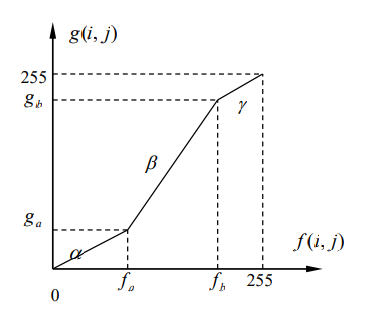
\includegraphics[width=0.5\linewidth]{screenshot036}
		\caption{对比度线性变换关系}
		\label{fig:screenshot036}
	\end{figure}
	
	设原图像的灰度为$f(i, j)$,处理后的图像的灰度为$g(i, j)$,对比度线性展宽的原理示意图如图1.1所示。假设原图像中我们关心的景物的灰度分布在$[f_{a},f_{b}]$区间内,处理后的图像中,我们关心的景物的灰度分布在$[g_{a}, g_{b}]$区间内。在这里 $\Delta g = (g_{b}-g_{a})>\Delta f=(f_{b}-f_{a})$,也就是说我们所关心的景物的灰度级得到了展宽。根据图中所示的映射关系中分段直线的斜率我们可以得出线性对比度展宽的计算公式:

	\begin{figure}[H]
		\centering
		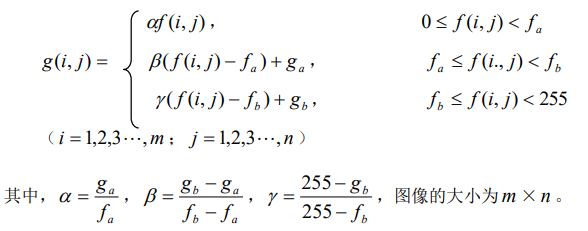
\includegraphics[width=0.7\linewidth]{screenshot040}
		\caption{线性对比度展宽公式}
		\label{fig:screenshot040}
	\end{figure}

	
	2. 直方图均衡化
	
	灰度直方图反映了数字图像中每一灰度级与其出现频率间的关系,它能描述图像的概貌。通过修改直方图的方法增强图像是一种实用而有效的处理技术。直方图均衡化是将原始图像通过某种变换,得到一幅灰度直方图为均匀分布的新图像的方法。  
	 
	离散图像均衡化处理可通过变换函数实现:

	\begin{equation}
		s_{k} = T(r_{k})=\Sigma n_{j}/n
	\end{equation}
	
	\subsection{实验内容、结果与分析}
	1.熟悉MATLAB语言中数字图像处理函数的使用。
	
	2. 图像灰度线性变换的实现
	
	(1)读入一幅灰度图像test1,显示其灰度直方图,实验结果如下图\ref{fig:1-3}所示,可以看到图像的灰度值大多分布在较小的灰度范围内,因此整个图像偏暗,这是笔者在江苏进行生产实习时,在宿舍拍的苏州夜景。
	
	\begin{figure}[H]
		\centering
		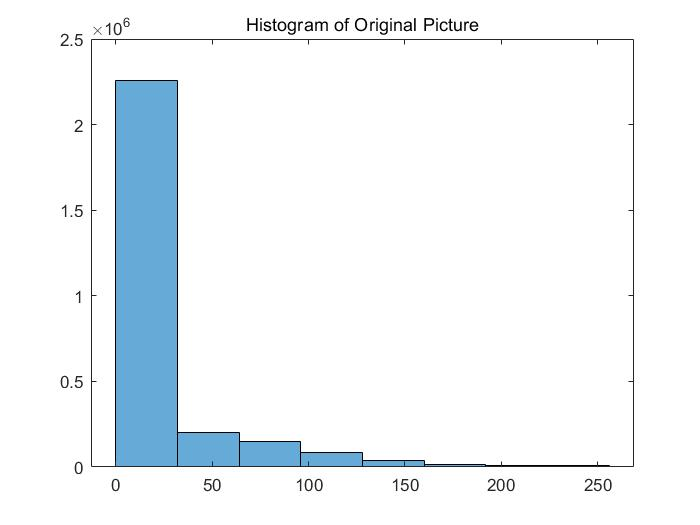
\includegraphics[width=0.5\linewidth]{1-3}
		\caption{图像的灰度直方图}
		\label{fig:1-3}
	\end{figure}

	(2)根据图像灰度直方图,选择所关心的图像景物的灰度分布范围$[f_{a},f_{b}]$,以及拟变换的灰度分布范围$[g_{a},g_{b}]$
	
	(3)实现对图像的灰度线性变换,可以看到对图像的较小灰度值范围线性变换到更大的范围内后,图像的对比度提高。在选择不同的变换范围时,整个图像的对比度相应的会发生变化,为了尽可能大地提高图像对比度,我们通常的做法不是寻找使图像对比度最大化的线性变换参数,而是使用更加普适的方法——图像直方图均衡化。
	\begin{figure}[H]
		\centering
		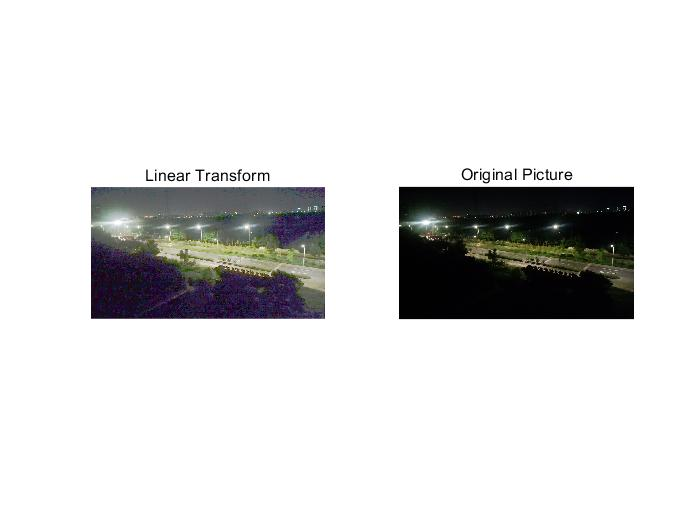
\includegraphics[width=0.7\linewidth]{1-1}
		\caption{线性变换得到的图像及其原图像}
		\label{fig:1-1}
	\end{figure}
	
	(4)调整$\alpha$,$\beta$,$\gamma$ 的值,观察对处理结果的影响。
	
	3. 图像的均衡化处理
	
	(1)读入一幅灰度图像test2,求出其直方图
	
	(2)利用Matlab函数实现图像的均衡化处理,关于图像直方图的均衡化之前一直都没有非常直观的理解,我觉得对于一些图像处理的基本原理和概念,特别不能以填鸭式的方法教学,不然在进行研究时始终都不得要领,在长时间的摸爬滚打之后获得对于这些知识的理解,无疑是一种巨大的代价。直方图均衡化理解csdn博客:\url{https:blog.csdn.net/qq_15971883/article/details/88699218}
	
	(3)同屏显示处理前后的图像和灰度直方图,说明处理前后直方图的变化以及对应的灰度变化,如下图所示,将之前的较暗的夜景图进行直方图均衡化之后,均衡化后的图像及其直方图如图\ref{fig:1-2}所示
	\begin{figure}[H]
		\centering
		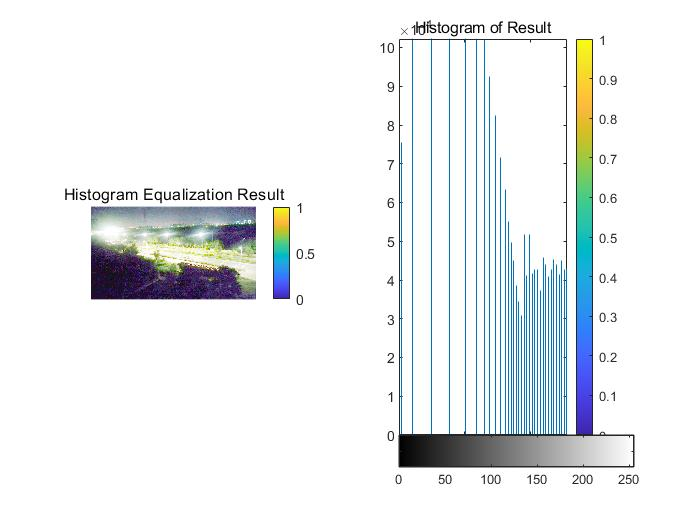
\includegraphics[width=0.5\linewidth]{1-2}
		\caption{夜景图直方图均衡化之后的图像及其直方图}
		\label{fig:1-2}
	\end{figure}

	\subsection{实验关键代码}
	\begin{lstlisting}[style=Matlab-editor]
		% clear
		clear all; close all; clc;
		
		pic = imread("darksense.jpg");
		
		g_a = 90; g_b =175;
		f_a = 5; f_b = 75;
		alpha = g_a/f_a;
		beta = (g_b-g_a)/(f_b-f_a);
		gama = (255-g_b)/(255-f_b);
		
		%% linear tran
		% 将pic矩阵分为满足三个区间的三个矩阵
		pic1 = double(pic).*alpha.*(pic<f_a);
		pic2 = (beta.*(double(pic)-f_a)+g_a).*((f_a<=pic) & (pic<f_b));
		pic3 = (gama.*(double(pic)-f_b)+g_b).*(f_b<=pic);
		
		% 矩阵叠加得到最终图像
		pic_result = uint8(pic1+pic2+pic3);
		figure(1);
		subplot(1, 2, 1);
		imshow(pic_result);
		title("Linear Transform");
		colorbar;
		
		subplot(1, 2, 2);
		imshow(pic);
		title("Original Picture");
		colorbar;
		
		
		%% histogram equalization
		figure(2);
		[J, T] = histeq(pic);
		subplot(1, 2, 1);
		imshow(J);
		title("Histogram Equalization Result");
		colorbar;
		
		subplot(1, 2, 2);
		imhist(J);
		title("Histogram of Result");
		colorbar;
		
		figure(3);
		histogram(pic, 8);
		title("Histogram of Original Picture");
		colorbar;
	\end{lstlisting}

	\subsection{实验思考}
	1.在映射关系中,分段直线的斜率的大小对图像处理结果有哪些影响?
	
	在线性变换中,实际上分段直线的斜率取决于变换前后的像素灰度值区间,当灰度区间从小向大变换时,使得各个像素值从小区间线性映射到大区间,像素之间的对比度增大,而这些像素值之间的相对大小没有改变,因此图像不会有太大的失真,明显的有利的效果时使得关注区域的图像对比度变大。同理,当灰度取键从大向小变换时,即压缩该区间的图像对比度,从反面的角度来看增大了两侧灰度区间的图像对比度。
	
	中间的协律和两侧变换的斜率是呈反比的关系的。
	
	当$\beta$大于1时,表示从关心区域从小区间映射到大区间,反之,表示关心区域从小区间映射到大区间。因此中间图像斜率$\beta$越大时,关心区域图像对比度增大,因为往往我们取得关系区域是图像大部分像素的区间,因此一般可以认为整个图像的对比度增大,反之同理。
	
	所以数字图像的像素值是一种有效的图像对比度变换的方法。
	
	2.在进行对比度扩展时,如果确定和选取所关心的景物?
	
	像素值线性变换的大部分问题在1中已经讨论的很充分了,在做对比度扩展时,必不可少的环节是对数字图像的直方图的绘制,直方图直接反映了图像像素值的分布,即反映了我们所关心的图像内容的主要集中范围。所以我们选取直方图像素集中的区域。
	
	3. 直方图均衡化适用于什么形式的灰度分布情形?

	原图较暗且动态范围小,在直方图中的表现是直方图灰度范围窄且集中在低灰度值区域。	

	\section{实验二:数字图像的傅里叶变换及其性质}
	\subsection{实验目的}
	1. 熟悉图像空间域和频率域的关系,掌握快速傅里叶变换
	
	2. 掌握离散傅里叶变换的性质和应用
	
	\subsection{实验原理}
	图像既能在空间域处理,也能在频率域处理。把图像信息从空域变换到频域,可以更好地分析、加工和处理
	\begin{figure}[H]
		\centering
		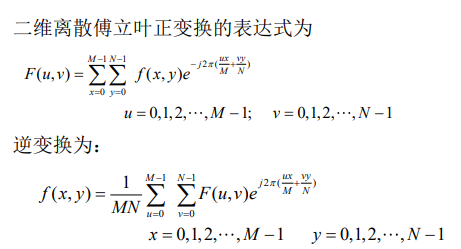
\includegraphics[width=0.7\linewidth]{screenshot037}
		\caption{二维傅里叶变换}
		\label{fig:screenshot037}
	\end{figure}

	二维离散傅立叶变换具有若干性质,如:线性性、平移性、可分离性、周期性、共轭对称性、旋转不变性等。
	
	\subsection{实验内容、结果与分析}
	1.产生一幅如图所示亮块图像$f(x,y)$(500×500 大小、暗处=0,亮处=255),产生的图像如图\ref{fig:2-1}所示。
	\begin{figure}[H]
		\centering
		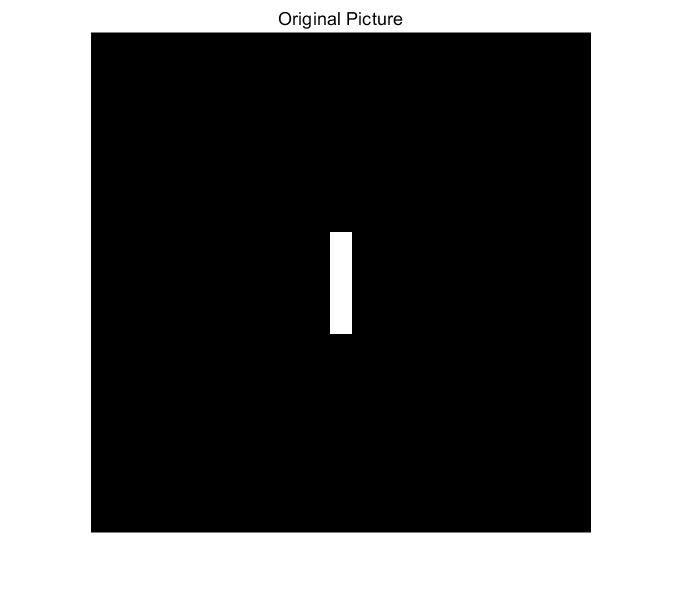
\includegraphics[width=0.5\linewidth]{2-1}
		\caption{原始亮块图像}
		\label{fig:2-1}
	\end{figure}
	
	(1)对其进行二维傅里叶变换,同屏显示原图f 和其傅里叶变换幅度谱图,如下图\ref{fig:2-2}所示,值得注意的是,此处的幅度谱图的分布是这样的:中心有主极大,亮度最强,占据整个频谱面的绝大部分能量,而向上下左右四侧都出现部分次极大,次极大的强度随着离中心的距离越远,强度越小。并且,由于原始图像是可以看成为竖立的矩形,因此在水平方向的频谱次极大强度强于垂直方向的频谱次极大强度。
	\begin{figure}[H]
		\centering
		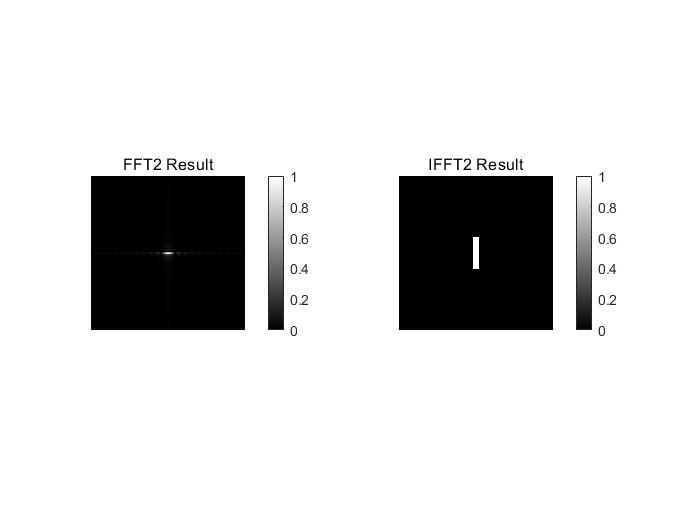
\includegraphics[width=0.7\linewidth]{2-2}
		\caption{原始图像与其傅里叶变换幅度谱图}
		\label{fig:2-2}
	\end{figure}
	
	(2)若令$f_{1}(x,y)=(-1)^{x+y}* f(x,y)$,重复以上过程,比较二者幅度谱的异同,简述理由,没搞懂。
	\begin{figure}[H]
		\centering
		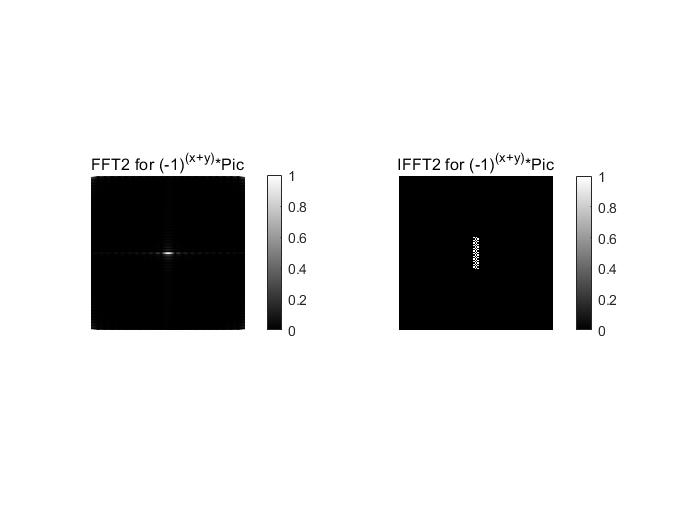
\includegraphics[width=0.7\linewidth]{2-3}
		\caption{将原图变换之后,得到的图像及其幅度谱}
		\label{fig:2-3}
	\end{figure}
	
	(3)若将$f(x,y)$顺时针旋转45度得到$f_{2}(x,y)$,试求出并显示$f_{2}(x,y)$的傅里叶幅度谱,并与$f(x,y)$的幅度谱进行比较和说明。在空间域内,图像做了45度的旋转,相当于乘以45度的相位因子,在频域内表现为位移(也看似旋转),所以最终的效果是频谱幅度谱同样发生旋转。
	\begin{figure}[H]
		\centering
		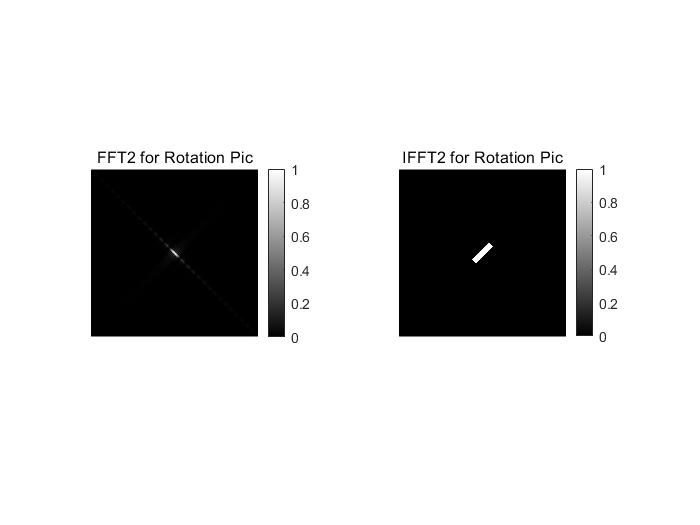
\includegraphics[width=0.7\linewidth]{2-4}
		\caption{将原始图像顺时针旋转45度得到的图像及其傅里叶幅度谱}
		\label{fig:2-4}
	\end{figure}
	
	
	2. 读入一幅数字图像test6
	
	(1)对其进行二维傅里叶变换,显示其傅里叶变换的幅度谱和相位谱。
	\begin{figure}[H]
		\centering
		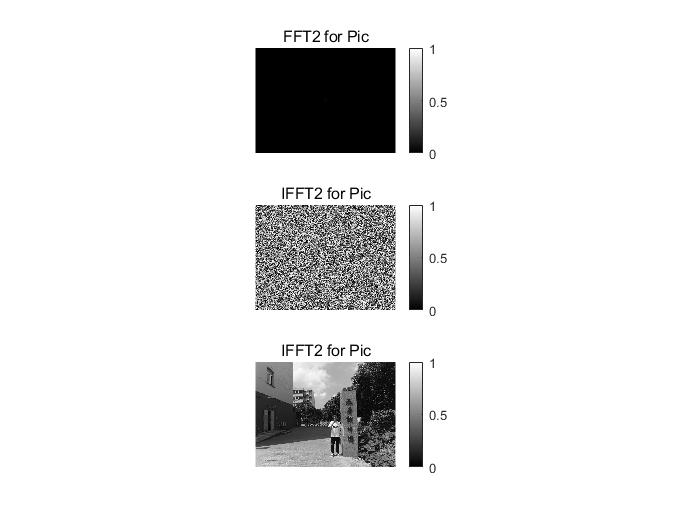
\includegraphics[width=0.7\linewidth]{2-5}
		\caption{读入的图像,及其傅里叶变换幅度谱与相位谱}
		\label{fig:2-5}
	\end{figure}
	
	
	(2)令其幅度谱为常数A,仅利用相位谱反傅里叶变换重建原图像,说明重建图像的特点。相位重建图中,恢复出了关键形状信息,相应的灰度信息丢掉了。
	
	(3)令相位谱为0,仅利用幅度谱进行反傅里叶变换重建原图像,分析说明重建图像的特点。我们可以看到它仅包含灰度信息,图像中没有形状信息
	
	(4)使用题1的幅度谱与test6的相位谱进行反傅里叶变换,分析说明重建图像的特点。即灰度信息来自于前面的图像,而相位信息来自于真实图像,可以朦胧看出人的轮廓,但是灰度信息表现得不明显。可以看到确定一幅图像的特性内容时,相位起到支配作用。
	\begin{figure}[H]
		\centering
		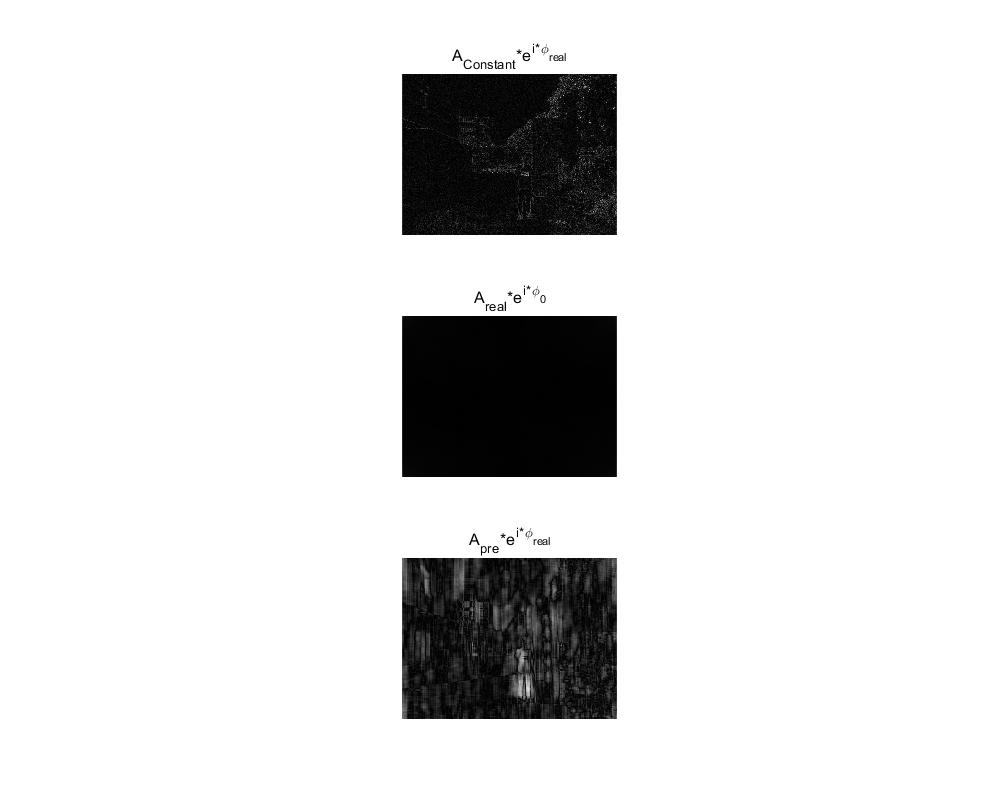
\includegraphics[width=0.7\linewidth]{2-6}
		\caption{在(2)、(3)、(4)三种情况下的重建图像}
		\label{fig:2-6}
	\end{figure}
	
	\subsection{实验关键代码}
	\begin{lstlisting}[style=Matlab-editor]
		% clear
		close all; clear all; clc
		
		pic = zeros(500, 500);
		pic(250-50:251+50, 250-10:251+10) = pic(250-50:251+50, 250-10:251+10)+255;
		pic = uint8(pic);
		
		figure(1);
		imshow(pic);
		title("Original Picture");
		
		%% 2D Fourier Transform(FFT) for pic
		% FFT for pic
		pic_fre = fft2(im2double(pic));
		figure(2);
		
		subplot(1, 2, 1);
		imshow(mat2gray(abs(fftshift(pic_fre))));
		title("FFT2 Result");
		colorbar;
		
		subplot(1, 2, 2);
		imshow(mat2gray(abs(ifft2(pic_fre))));
		title("IFFT2 Result");
		colorbar;
		
		%% FFT for (-1)^(x+y)*Pic
		pic1 = pic;
		pic1(1:2:end, 2:2:end) = -pic(1:2:end, 1:2:end);
		pic1(2:2:end, 1:2:end) = -pic(2:2:end, 2:2:end);
		pic1_fre = fft2(im2double(pic1));
		
		figure(3);
		subplot(1, 2, 1)
		imshow(mat2gray(abs(fftshift(pic1_fre))));
		title("FFT2 for (-1)^{(x+y)}*Pic");
		colorbar;
		
		subplot(1, 2, 2)
		imshow(mat2gray(abs(ifft2(pic1_fre))));
		title("IFFT2 for (-1)^{(x+y)}*Pic");
		colorbar;
		
		%% clock wise rotate pi/2
		pic2 = imrotate(pic, -45);
		pic2_fre = fft2(im2double(pic2));
		
		figure(4);
		subplot(1, 2, 1)
		imshow(mat2gray(abs(fftshift(pic2_fre))));
		title("FFT2 for Rotation Pic");
		colorbar;
		
		subplot(1, 2, 2)
		imshow(mat2gray(abs(ifft2(pic2_fre))));
		title("IFFT2 for Rotation Pic");
		colorbar;
		
		%% FFT for real image
		pic4 = imread("person.jpg");
		pic4 = im2gray(pic4);
		pic4_fre = fft2(im2double(pic4));
		
		figure(5);
		subplot(3, 1, 1)
		imshow(mat2gray(abs(fftshift(pic4_fre))));
		title("FFT2 for Pic");
		colorbar;
		
		subplot(3, 1, 2)
		imshow(mat2gray(angle(fftshift(pic4_fre))*180/pi));
		title("IFFT2 for Pic");
		colorbar;
		
		subplot(3, 1, 3);
		imshow(mat2gray(abs(ifft2(pic4_fre))));
		title("IFFT2 for Pic");
		colorbar;
		
		%% different combination
		A = 10;
		pic4_fre1 = A*exp(1i*angle(pic4_fre));
		pic4_fre2 = abs(pic4_fre)*exp(1i*0);
		pic4_fre3 = imresize(abs(pic_fre),"OutputSize", size(angle(pic4_fre), [1 2])).*exp(1i*angle(pic4_fre));
		
		figure(6);
		subplot(3, 1, 1);
		imshow(im2uint8(mat2gray(abs(ifft2(pic4_fre1)))));
		title("A_{Constant}*e^{i*\phi_{real}}");
		
		subplot(3, 1, 2);
		imshow(im2uint8(mat2gray(abs(ifft2(pic4_fre2)))));
		title("A_{real}*e^{i*\phi_{0}}");
		
		subplot(3, 1, 3);
		imshow(im2uint8(mat2gray(abs(ifft2(pic4_fre3)))));
		title("A_{pre}*e^{i*\phi_{real}}");
	\end{lstlisting}
	
	\subsection{实验思考}
	1.在傅里叶反变换中,幅度谱和相位谱对重建图像的影响分别体现在什么方面?
	对于自然图像,相位包含了更多的视觉信息,表征图像的形状,而幅度表征的灰度信息难以理解和表征。来自知乎的讨论\url{https://www.zhihu.com/question/23718291}
	
	\section{实验三:数字图像的空间域和频率域增强}
	\subsection{实验目的}
	1. 熟悉图像空间域增强方法,掌握增强模板使用方法
	
	2. 掌握均值滤波器、中值滤波器的理论基础和实现方法
	
	3. 掌握频率域滤波的基本理论和实现方法
	
	\subsection{实验原理}
	图像增强是数字图像处理的基本内容之一,其目的是根据应用需要突出图像中的某些“有用”信息,削弱或去除不需要的信息,以改善图像的视觉效果,或突出图像的特征,便于计算机处理。图像增强可以在空间域进行,也可以在频率域中进行。
	
	1.空间域增强滤波
	
	空间域滤波主要利用空间模板进行,如$3*3$,$5*5$模板等。
	
	一般来说,使用大小为m×n 的滤波器对大小为M×N 的图像f进行空间滤波,可表示成: 
	\begin{figure}[H]
		\centering
		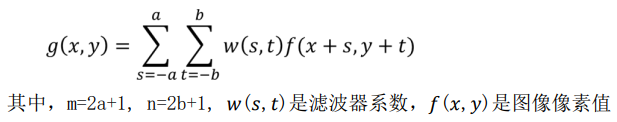
\includegraphics[width=0.7\linewidth]{screenshot038}
		\caption{空间滤波数学表达}
		\label{fig:screenshot038}
	\end{figure}

	均值滤波器是一种空间平滑滤波器,它是对包含噪声的图像上的每个像素点,用它邻域内像素的平均值替代原来的像素值。例如,采用一个$3×3$的模板,待处理的像素为$f(i,j)$,则处理后图像对应的像素值为
	\begin{equation}
		g(i,j)=1/9*(f(i-1,j-1)+f(i-1,j)+f(i-1,j+1)+f(i,j-1)//
		+f(i,j)+f(i,j+1)+f(i+1,j-1)+f(i+1,j)+f(i+1,j+1));  
	\end{equation}
   
	
	中值滤波器也是一种空间平滑滤波器,它是对以图像像素点为中心的一个滑动窗口内的诸像素灰度值排序,用中值代替窗口中心像素的原来灰度值,因此它是一种非线性的图像平滑法。
	
	空间域锐化可采用一阶微分算子,如梯度算子、Roberts、Prewitt和Sobel算子等,也可采用二阶Laplacian锐化算子,它们的目的都是突出图像的边缘或轮廓。微分算子也可以写成模板作用的形式,如二阶Laplacian锐化算子可写为:
	\begin{equation}
		g(i,j)=4*f(i,j)-(f(i-1,j-1)+f(i,j-1)+f(i,j+1)+f(i+1,j)); 
	\end{equation}

	
	其中,$f(i,j)$为待处理的像素值,$g(i,j)$为处理后图像对应的像素值。
	
	2. 频率域滤波
	
	图像频率域滤波可利用离散傅里叶变换,将图像信号从空间域变换到频率域,在频率域选择合适的滤波器$H(u,v)$对图像的频谱成分$F(u,v)$进行处理,然后经逆傅立叶变换得到处理图像,实现图像处理结果。频率域滤波的一般过程如下:
	\begin{figure}[H]
		\centering
		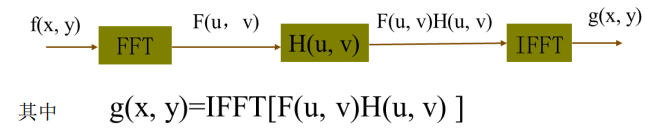
\includegraphics[width=0.7\linewidth]{screenshot039}
		\caption{频率域滤波的一般过程}
		\label{fig:screenshot039}
	\end{figure}
	
	由于噪声主要集中在高频部分,为去除噪声改善图像质量,图像平滑滤波采用低通滤波器$H(u,v)$来抑制高频成分,通过低频成分,达到平滑图像的目的。    而图像锐化是为了消除模糊,突出边缘和细节,因此采用高通滤波器让高频成分通过,使低频成分削弱,再经逆傅立叶变换得到边缘锐化的图像。
	
	\subsection{实验内容、结果与分析}
	1.读入一幅数字图像test3
	
	2. 图像的平滑滤波处理
	
	1)对原图像分别加入高斯噪声、椒盐噪声。
	\begin{figure}[H]
		\centering
		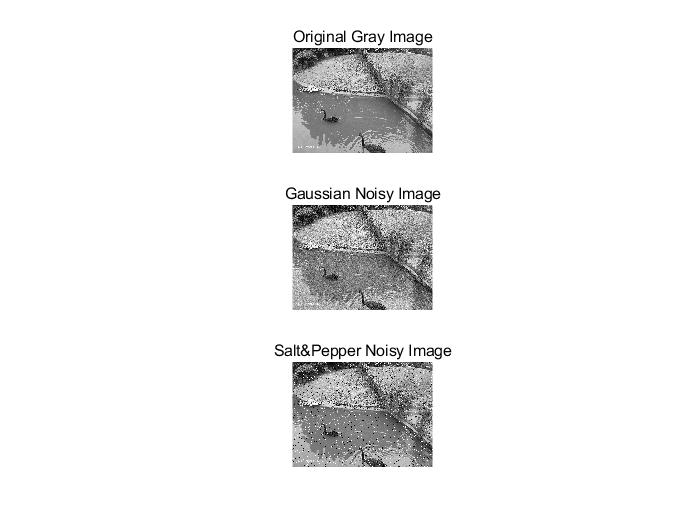
\includegraphics[width=0.7\linewidth]{3-1}
		\caption{加不同的噪声显示的图像}
		\label{fig:3-1}
	\end{figure}
	
	
	2)利用邻域平均法,分别采用$3*3$,$5*5$模板对加噪声图像进行平滑处理,显示原图像、加噪图像和处理后的图像。
	
	3)利用中值滤波法,分别采用$3*3$,$5*5$模板对加噪声图像进行去噪处理,显示原图像、加噪图像和处理后的图像。
	\begin{figure}[H]
		\centering
		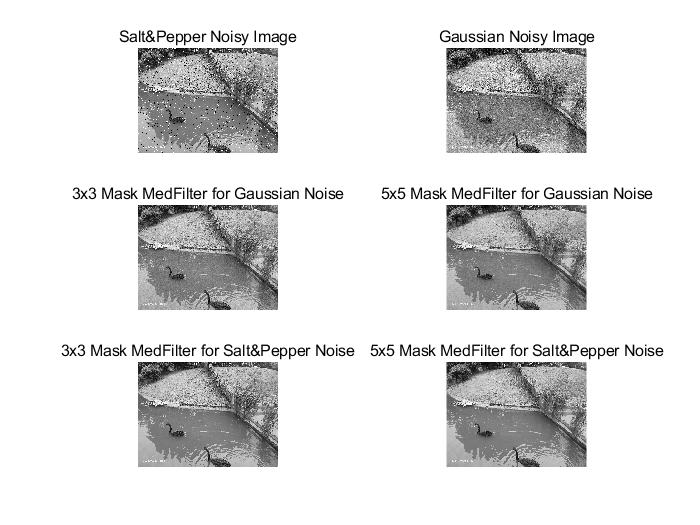
\includegraphics[width=0.7\linewidth]{3-2}
		\caption{使用模板大小的中值滤波方法得到的图像}
		\label{fig:3-2}
	\end{figure}

	\begin{figure}[H]
		\centering
		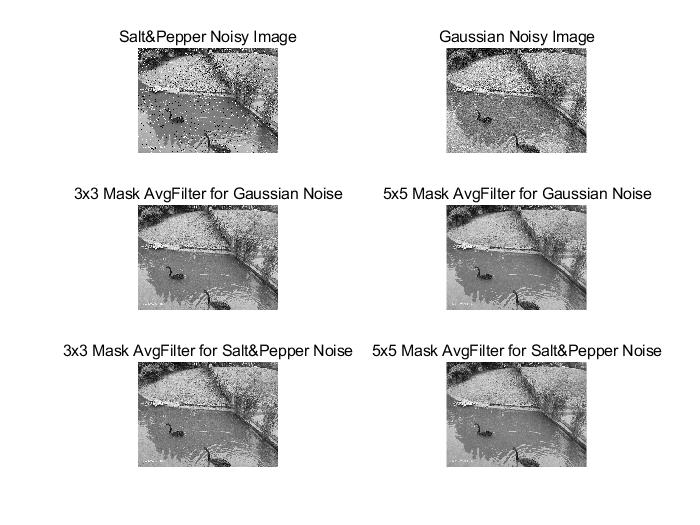
\includegraphics[width=0.7\linewidth]{3-3}
		\caption{使用模板大小的均值滤波方法得到的图像}
		\label{fig:3-3}
	\end{figure}
	
	
	4)比较各种滤波方法和滤波模板的处理结果,并分析说明。
	
	中值滤波法顾名思义就是在某个模板/滤波器/核/mask里面的像素值,对其按照大小顺序排列(大到小/小到大),取其中位数为其滤波器作用的像素点的新值。而均值滤波器即使用某个滤波器内所有像素点的均值作为该滤波器作用的像素点的新值。值得注意的是,所有的这种空间滤波方法在使用模板/滤波器/核/mask时,都要考虑填充方法,即padding,padding在图像处理中是一个基本概念,学习过卷积神经网络(CNN)的应该知道,在做卷积层,就有padding,一般这里选用的是zero padding。当然也有其他的填充方法。关于padding在深度学习中的作用,参考知乎博客:\url{https://zhuanlan.zhihu.com/p/36278093}
	
	当使用不同的模板大小作用时,一般我们称这个模板大小范围为感受野,在DL中做图像处理是,感受野越大,新像素值的相关范围越大,考虑的因素也就越多,但是付出的代价是,要么计算量增大;要么难以获得足够细致的图像细节部分。在这里也是有异曲同工之妙。
	
	3. 读入一幅数字图像test5,选择适当的滤波半径,在频域分别进行理想低通、理想高通、高斯低通、高斯高通滤波,显示原始图像及它的傅里叶幅度谱图,以及低通、高通滤波后的结果图像及它们的傅里叶幅度谱,分析说明滤波处理后图像与原始图像的区别。
	
	此处的参考博客:\url{https://blog.csdn.net/u010936286/article/details/80299959?ops_request_misc=&request_id=&biz_id=102&utm_term=matlab%20%E4%BD%BF%E7%94%A8%E7%9B%B8%E4%BD%8D%E5%92%8C%E6%8C%AF%E5%B9%85%E9%87%8D%E5%BB%BA%E5%9B%BE%E5%83%8F%20%E5%86%88%E8%90%A8%E9%9B%B7%E6%96%AF&utm_medium=distribute.pc_search_result.none-task-blog-2~all~sobaiduweb~default-0-80299959.first_rank_v2_pc_rank_v29&spm=1018.2226.3001.4187}
	\begin{figure}[H]
		\centering
		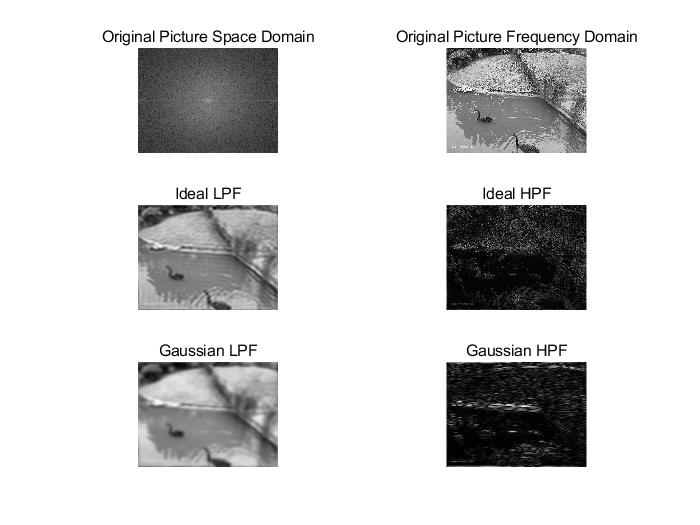
\includegraphics[width=0.7\linewidth]{3-4}
		\caption{使用不同的频域滤波器实现的滤波效果}
		\label{fig:3-4}
	\end{figure}
	
	\subsection{实验关键代码}
	\begin{lstlisting}[style=Matlab-editor]
		% clear 
		% copyrighy@zhoumi
		close all; clear all; clc
		
		pic = imread("goose.jpg");
		pic = im2gray(pic);
		
		%% add some noise
		pic_gn = imnoise(pic, "gaussian");
		pic_sn = imnoise(pic, "salt & pepper");
		
		figure(1);
		subplot(3, 1, 1);
		imshow(pic);
		title("Original Gray Image");
		
		subplot(3, 1, 2);
		imshow(pic_gn);
		title("Gaussian Noisy Image");
		
		subplot(3, 1, 3);
		imshow(pic_sn);
		title("Salt&Pepper Noisy Image");
		
		%% Medium Filtering
		pic_gn_medfil1 = medfilt2(pic_gn, [3 3], "symmetric");
		pic_gn_medfil2 = medfilt2(pic_gn, [5 5], "symmetric");
		
		pic_sn_medfil1 = medfilt2(pic_sn, [3 3], "symmetric");
		pic_sn_medfil2 = medfilt2(pic_sn, [5 5], "symmetric");
		
		figure(2);
		subplot(3, 2, 1);
		imshow(pic_sn);
		title("Salt&Pepper Noisy Image");
		
		subplot(3, 2, 2);
		imshow(pic_gn);
		title("Gaussian Noisy Image");
		
		subplot(3, 2, 3);
		imshow(pic_gn_medfil1);
		title("3x3 Mask MedFilter for Gaussian Noise");
		
		subplot(3, 2, 4);
		imshow(pic_gn_medfil2);
		title("5x5 Mask MedFilter for Gaussian Noise");
		
		subplot(3, 2, 5);
		imshow(pic_sn_medfil1);
		title("3x3 Mask MedFilter for Salt&Pepper Noise");
		
		subplot(3, 2, 6);
		imshow(pic_sn_medfil2);
		title("5x5 Mask MedFilter for Salt&Pepper Noise");
		
		%% Average Filtering
		pic_gn_medfil1 = filter2(fspecial('average',3), pic_gn)/255;
		pic_gn_medfil2 = filter2(fspecial('average',5), pic_gn)/255;
		
		pic_sn_medfil1 = filter2(fspecial('average',3), pic_sn)/255;
		pic_sn_medfil2 = filter2(fspecial('average',5), pic_sn)/255;
		
		figure(3);
		subplot(3, 2, 1);
		imshow(pic_sn);
		title("Salt&Pepper Noisy Image");
		
		subplot(3, 2, 2);
		imshow(pic_gn);
		title("Gaussian Noisy Image");
		
		subplot(3, 2, 3);
		imshow(pic_gn_medfil1);
		title("3x3 Mask MedFilter");
		
		subplot(3, 2, 4);
		imshow(pic_gn_medfil2);
		title("5x5 Mask MedFilter");
		
		subplot(3, 2, 5);
		imshow(pic_sn_medfil1);
		title("3x3 Mask MedFilter for Salt&Pepper Noise");
		
		subplot(3, 2, 6);
		imshow(pic_sn_medfil2);
		title("5x5 Mask MedFilter for Salt&Pepper Noise");
		
		%% Filtering in Frequency Domain
		pic_fre = fft2(im2double(pic));
		
		lpf = zeros(size(pic_fre));
		range = 25;
		lpf(size(lpf, 1)/2-range:size(lpf, 1)/2+range+1, size(lpf, 2)/2-range:size(lpf, 2)/2+range+1) = 1;
		hpf = 1-lpf;
		
		glf = fspecial('gaussian',size(pic_fre), 15);
		ghf = max(glf)-glf;
		
		pic_re1 = im2uint8(mat2gray(abs(ifft2(fftshift(fftshift(pic_fre).*lpf)))));
		pic_re2 = im2uint8(mat2gray(abs(ifft2(fftshift(fftshift(pic_fre).*hpf)))));
		pic_re3 = im2uint8(mat2gray(abs(ifft2(fftshift(fftshift(pic_fre).*glf)))));
		pic_re4 = im2uint8(mat2gray(abs(ifft2(fftshift(fftshift(pic_fre).*ghf)))));
		
		figure(4);
		subplot(3, 2, 1)
		imshow(mat2gray(abs(log(1+fftshift(pic_fre)))));
		title("Original Picture Space Domain");
		
		subplot(3, 2, 2);
		imshow(pic);
		title("Original Picture Frequency Domain");
		
		subplot(3, 2, 3);
		imshow(pic_re1);
		title("Ideal LPF");
		
		subplot(3, 2, 4);
		imshow(pic_re2);
		title("Ideal HPF");
		
		subplot(3, 2, 5);
		imshow(pic_re3);
		title("Gaussian LPF");
		
		subplot(3, 2, 6);
		imshow(pic_re4);
		title("Gaussian HPF");
	\end{lstlisting}
	
	\subsection{实验思考}
	1.采用均值滤波、中值滤波,对高斯噪声和椒盐噪声的抑制哪种比较有效?
	均值滤波器是一种最常用的线性低通平滑滤波器,可抑制图像中的加性噪声,但同时也使图像变得模糊;中值滤波器是一种最常用的非线性平滑滤波器,可消除图像中孤立的噪声点,又可产生较少的模糊。一般情况下中值滤波的效果要比邻域平均处理的低通滤波效果好,主要特点是滤波后图像中的轮廓比较清晰。
	
	因此,对于高斯噪声来说,使用均值滤波由于均值为0的条件,所以会获得比较好的效果,而中值滤波效果会稍差;对于椒盐噪声来说,噪声是一个突变值,使用中值滤波效果更好,均值滤波会引入较大的不必要的模糊。
	
	2.模板大小的不同,所处理效果有何不同?为什么?
	模板大小对处理效果的影响在实验二中提及,即感受野不同,对于均值滤波来说,图像会更加模糊,一种理解的极端情况是:模板的大小等于整个图像的大小,整个图像都模糊了。而对于中值滤波来说,相较于原图像来说,同样会造成一些失真,但是我们要对滤波带来的失真和对于噪声滤除造成的失真的消除做一个权衡,使得最终图像的效果达到最好的效果。
	
	3.频率域滤波在实现过程应如何处理? 
	频率域幅度谱中,在进行fftshift之后,中心的空间频率最小,为零,越向外围空间频率越大,离中心的距离表示频率的大小,而中心向外的向量方向表示频率的方向。
	
	低频信号占据图像的绝大部分能量,即低频分量占大多数,高频占少数。在图像中,高频分量表示图像中物体的轮廓,而像椒盐噪声一样的噪声一般是一个突变值,所以一般属于高频噪声,使用低通滤波器可以滤除。在数字滤波时,可以使用理想高通、低通滤波器,在物理实现时无法实现。
	
	在进行频域滤波时,先将图像变换到频域,然后与某频域滤波器的直接逐元素相乘,然后反二维傅里叶变换即可,与一维信号的频域滤波类似。

	\section{实验总结}
	\subsection{MATLAB数字图像常见处理}
	1. 实验结果图像对比度不强,要么太偏白,要么太偏暗
	
	使用$log(1+x)$对像素值进行变换,或者使用mat2gray对某些越界的像素值变换回要求的区间(如0-255)。\\
	
	2. 图像数据类型与转换
	
	直接读取图像得到的时uint8类型数据,在做傅里叶变换等数值运算时,需要事先使用im2double变换到double类型。\\
	
	对于图像来讲(比如做显示时),double类型数据位于0-1,uint8位于0-255,所以需要用到im2double、im2uint8等做变换。\\
	
	3. 图像的读取与显示、直方图、直方图均衡化
	
	imread函数、imshow函数、imresize函数、histogram函数、histeq函数\\
	
	4. 绘图:子图绘制、标题、坐标区限制、色标块
	
	subplot+imshow函数(如何控制子图大小还没有解决)、title函数、xLim和yLim函数、colorbar函数\\
	
	5. 图像二维傅里叶变换及其逆变换
	
	fft2函数、ifft2函数、fftshift函数、angle函数、abs函数\\
	
	6. 图像常用数字图像滤波器
	
	fspecial函数、filter2函数、medfilt2函数\\
	
	7. 一些其他的需要注意的MATLAB操作
	
	imnoise函数、im2gray函数\\
	
	\subsection{心得与体会}
	1. 建立自己的知识库
	
	学习完某一方面的知识,及时完成积累和知识库的建立,以免反复浪费时间。\\
	
	2. 对于二维傅里叶变换与光学的思考
	
	自己在学光学的东西,联想到:二维傅里叶变换等效于光学中的夫琅禾费衍射\\
	
	3. 对数字图像处理课程的建议
	
	多介绍机器学习和深度学习,特别是CNN中一些技巧。还有建立语音信号处理及自然语言处理相关RNN技巧。\\
	
	4. 关于" 关键代码小节 "的解释

	在这里报告的格式下,不同于论文,代码量有限的情况下,将整个处理代码粘上我认为利远远大于弊\\
	
	5.  数字图像处理的收获
	
	巩固课堂知识,练习数字图像处理相关编程方法\\

\end{document}